\chapter{Koekytkentälevyn käyttö}

\section{Rinnankytkentä}
Kahden kaksijalkaisen komponentin rinnankytkentä saadaan aikaan laittamalla molempien komponenttien toinen jalka yhdelle riville ja toiset jalat jollekin muulle riville:


\begin{minipage}{0.75\textwidth}
\begin{center}
Koekytkentälevyllä
\end{center}
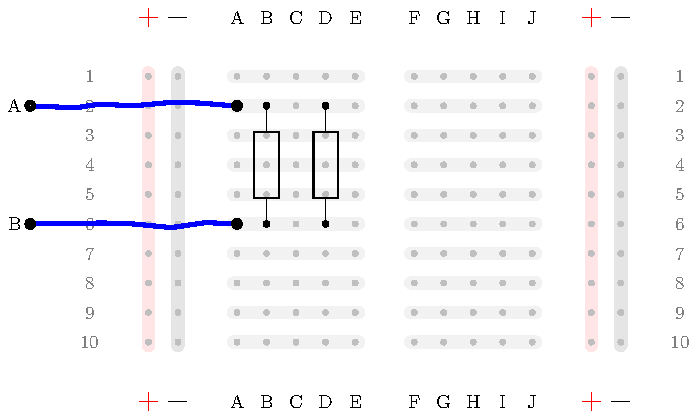
\includegraphics[width=0.8\textwidth]{kuvat/kuva1.pdf}
\end{minipage}%
\begin{minipage}{0.25\textwidth}
\begin{center}
Piirikaavio
\end{center}
\begin{tikzpicture}[scale=0.8]
%\draw (0,0) to[R] (0,5);
%\draw (3,0) to[R] (3,5);
\draw (0,0) node[anchor=east] {B} to[short, o-] (1,0) to[R,*-*] (1,2) -- (3,2) to[R] (3,0) -- (1,0) (1,2) to[short, -o] (0,2) node[anchor=east]{A};
\end{tikzpicture}
\end{minipage}
\begin{tcolorbox}[colback=yellow!10, title={Testaa taitosi!},colbacktitle=orange]
Piirrä toinen kaksijalkainen komponentti jo piirretyn komponentin rinnalle. Piirrä myös pisteet A ja B kuvaan.

\begin{tikzpicture}[scale=0.45]
\BREADBOARD (0,0) {10};
\draw (C3) to[R,*-*] (C7);
\unless\ifHideSolutions
\draw (E3) to[R,*-*] (E7);
\draw[blue,wire] (A3) to[short,*-o] ++(-7,0) node[left,black] {A};
\draw[blue,wire] (A7) to[short,*-o] ++(-7,0) node[left,black] {B};
\fi

\end{tikzpicture}\\
\begin{solution}
Kuvassa on esitetty yksi esimerkki, mutta myös muita vaihtoehtoja on olemassa.
\end{solution}
\end{tcolorbox}

%\clearpage
\section{Sarjaankytkentä}
Kahden kaksijalkaisen komponentin sarjankytkentä saadaan aikaan laittamalla molempien komponenttien toinen jalka yhdelle riville ja toiset jalat kahdelle muulle riville: 

\begin{minipage}{0.8\textwidth}
\begin{center}
Koekytkentälevyllä
\end{center}
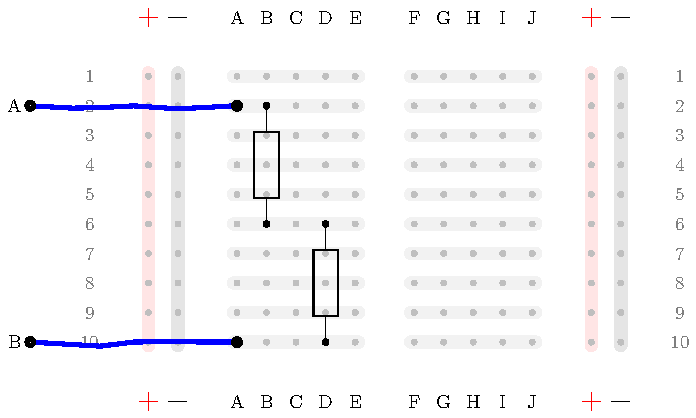
\includegraphics[width=0.9\textwidth]{kuvat/kuva2.pdf}
\end{minipage}
\begin{minipage}{0.2\textwidth}
Piirikaavio\\
\begin{tikzpicture}
%\draw (0,0) to[R] (0,5);
%\draw (3,0) to[R] (3,5);
\draw (0,0.5) node[anchor=east] {B} to[short, o-] (0,1) to[R] (0,3)--(0,3.5) to[R] (0,5.5) to[short,-o] (0,6) node[anchor=west]{A};
\end{tikzpicture}
\end{minipage}


\begin{tcolorbox}[colback=yellow!10, title={Testaa taitosi!},colbacktitle=orange]
Piirrä toinen kaksijalkainen komponentti jo piirretyn komponentin kanssa sarjaan. Piirrä myös pisteet A ja B kuvaan. 

\begin{tikzpicture}[scale=0.5][remember picture]
\BREADBOARD (0,0) {10};
\draw (C1) to[R,*-*] (C5);
\unless\ifHideSolutions
\draw (B5) to[R,*-*] (B9);
\draw[blue,wire] (A1) to[short,*-o] ++(-7,0) node[left,black] {A};
\draw[blue,wire] (A9) to[short,*-o] ++(-7,0) node[left,black] {B};
\fi

\end{tikzpicture}\\
\begin{solution}
Kuvassa on esitetty yksi esimerkki, mutta myös muita vaihtoehtoja on olemassa.
\end{solution}
\end{tcolorbox}

\section{Useampi kaksijalkainen komponentti piirissä}

Harjoitellaan vielä useamman komponentin kytkentää koekytkentälevylle. Nyt, jotta pysytään paremmin perillä, käytetään numeroita komponenttien vieressä, jotta muistetaan mikä komponentti on kyseessä.

\begin{center}
Piirikaavio\\
\begin{tikzpicture}

\draw (0,0) node[anchor=east] {B} to [short, o-*] (1,0) to[R=$R_1$,*-] (1,2)--(2,2) to[R=$R_2$] (2,0) -- (1,0);

\draw (0,2) node[anchor=east] {A} to [short,o-*] (1,2);
\draw (2,2) to[R=$R_3$,*-] (4,2) to[short,-o] (5,2) node[right] {C};
\end{tikzpicture}

Koekytkentälevyllä\\
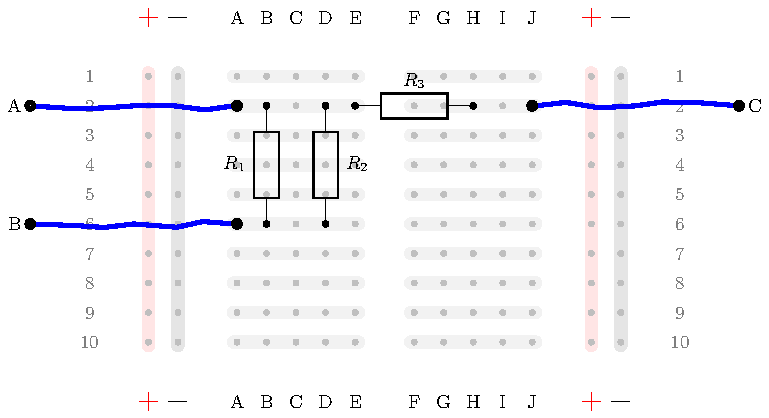
\includegraphics[width=0.95\textwidth]{kuvat/kuva3.pdf}
\end{center}


\begin{tcolorbox}[colback=yellow!10, title={Testaa taitosi!},colbacktitle=orange]
Piirrä kuvan mukainen kytkentä koekytkentälevylle.
\centering
\begin{tikzpicture}
\draw (0,0) node[anchor=east] {B} to [short, o-] (1,0) to[R=$R_1$] (1,2);

\draw (0,2) node[anchor=east] {A} to [short,o-*] (1,2);
\draw (1,2) to[R=$R_2$,*-] (4,2) to[short,-o] (6,2) node[right] {C};
\draw (4,2) to[R,a=$R_3$,*-] (4,0) --(5,0) to[R,a=$R_4$,*-*] (5,2);
\draw (5,0) to[short,-o] (6,0) node[right] {D};
\end{tikzpicture}

\begin{tikzpicture}[scale=0.5]
\BREADBOARD (0,0) {15};

\unless\ifHideSolutions
\draw (B10) to[R=$R_1$,*-*] (B14);
\draw[blue,wire] (A10) to[short,*-o] ++(-7,0) node[left,black] {A};
\draw[blue,wire] (A14) to[short,*-o] ++(-7,0) node[left,black] {B};
\draw (C10) to[R=$R_2$,*-*] (C6);
\draw (B6) to [R=$R_3$,*-*] (B2);
\draw (D6) to [R=$R_4$,*-*] (D2);
\draw[blue,wire] (A6) to[short,*-o] ++(-7,0) node[left,black] {C};
\draw[blue,wire] (A2) to[short,*-o] ++(-7,0) node[left,black] {D};
\fi

\end{tikzpicture}\\
\begin{solution}
Kuvassa on esitetty yksi esimerkki, mutta myös muita vaihtoehtoja on olemassa.
\end{solution}
\end{tcolorbox}

\begin{tcolorbox}[colback=yellow!10, title={Testaa taitosi!},colbacktitle=orange,]
Merkitse koekytkentälevylle johdot solmuihin A, B, C ja D.

\centering
\begin{tikzpicture}
\draw (0,0) node[anchor=east] {A} to [short, o-] (1,0) to[R=$R_1$] (1,2);
\draw (0,3) node[anchor=east] {B} to [short,o-*] (1,3);
\draw (1,2) to[R=$R_2$,*-] (4,2) to[short,-o] (6,2) node[right] {C};
\draw (1,2) to[short,*-] (1,3) to[R=$R_3$] (4,3) to[short,-*] (4,2);
\draw (4,2) to[R,a=$R_4$,*-] (4,0) --(5,0) to[R,a=$R_5$,*-*] (5,2);
\draw (5,0) to[short,-o] (6,0) node[right] {D};
\end{tikzpicture}

\begin{tikzpicture}[scale=0.5]
\BREADBOARD (0,0) {15};

\draw (B10) to[R=$R_1$,*-*] (B14);
\draw (C10) to[R=$R_2$,*-*] (C6);
\draw (E10) to[R,a=$R_3$,*-*] (E6);
\draw (B6) to [R=$R_4$,*-*] (B2);
\draw (D6) to [R,a=$R_5$,*-*] (D2);
\unless\ifHideSolutions

\draw[blue,wire] (A10) to[short,*-o] ++(-7,0) node[left,black] {B};
\draw[blue,wire] (A14) to[short,*-o] ++(-7,0) node[left,black] {A};

\draw[blue,wire] (A6) to[short,*-o] ++(-7,0) node[left,black] {C};
\draw[blue,wire] (A2) to[short,*-o] ++(-7,0) node[left,black] {D};
\fi

\end{tikzpicture}\\
\begin{solution}
Kuvassa on esitetty yksi esimerkki, mutta myös muita vaihtoehtoja on olemassa.
\end{solution}
\end{tcolorbox}


\begin{tcolorbox}[colback=yellow!10, title={Testaa taitosi!},colbacktitle=orange]
Jos edelliseen piiriin pitäisi lisätä vastus olemassa olevan solmun D ja uuden solmun E välille, mihin väliin kytkisit uuden vastuksen?

\begin{tikzpicture}[scale=0.5]
\BREADBOARD (0,0) {15};

\draw (B10) to[R=$R_1$,*-*] (B14);
\draw (C10) to[R=$R_2$,*-*] (C6);
\draw (E10) to[R,a=$R_3$,*-*] (E6);
\draw (B6) to [R=$R_4$,*-*] (B2);
\draw (D6) to [R,a=$R_5$,*-*] (D2);
\unless\ifHideSolutions
\draw (E2) to [R=R,*-*] (H2);
\draw[blue,wire] (A10) to[short,*-o] ++(-7,0) node[left,black] {B};
\draw[blue,wire] (A14) to[short,*-o] ++(-7,0) node[left,black] {A};

\draw[blue,wire] (A6) to[short,*-o] ++(-7,0) node[left,black] {C};
\draw[blue,wire] (A2) to[short,*-o] ++(-7,0) node[left,black] {D};
\draw[blue,wire] (J2) to[short,*-o] ++(7,0) node[right,black] {E};
\fi

\end{tikzpicture}\\
\begin{solution}
Kuvassa on esitetty yksi esimerkki, mutta myös muita vaihtoehtoja on olemassa.

\centering
\begin{tikzpicture}
\draw (0,0) node[anchor=east] {A} to [short, o-] (1,0) to[R=$R_1$] (1,2);
\draw (0,3) node[anchor=east] {B} to [short,o-*] (1,3);
\draw (1,2) to[R=$R_2$,*-] (4,2) to[short,-o] (6,2) node[right] {C};
\draw (1,2) to[short,*-] (1,3) to[R=$R_3$] (4,3) to[short,-*] (4,2);
\draw (4,2) to[R,a=$R_4$,*-] (4,0) --(5,0) to[R,a=$R_5$,*-*] (5,2);
\draw (5,0) to[short,-o] (6,0) node[right] {D};
\draw (5,0) to[short] (5,-0.5) to[R,a=R] (7,-0.5) to[short,-o] (8,-0.5) node[below] {E}; 
\end{tikzpicture}

\end{solution}
\end{tcolorbox}

\clearpage
\section{Koekytkentälevystä}

\begin{itemize}
    \item Yksi rivi (A-B-C-D-E) tai (F-G-H-I-J) vastaa yhtä solmua piirroksessa.
    \item Jos yhteen solmuun kiinnittyy enintään viisi (5) viivaa, riittää käyttää kaikki valmiina olevat paikat (A-E tai F-J). 
    \item Jos yhdessä solmussa on yli viisi (5) viivaa, tee lisä tilaa lisäämällä johto (eli oikosulku) esimerkiksi saman rivin toiselle puolelle (esimerkiksi käytössä rivi 3: kytke johto E3:sta F3:een, ja sinulla on nyt vapaana A3, B3, C3, D3, G3, H3, I3 ja J3.
    \item $+$ tai $-$ pystyrivejä käytetään yleensä käyttöjännitteelle (punainen $+$) sekä maalle (musta $-$). Näistä lisää seuraavaksi.
\end{itemize}

\begin{center}
\begin{tikzpicture}[scale=0.5]
\BREADBOARD (0,0) {15};
\end{tikzpicture}
\end{center}

\section{Ensimmäinen kytkentä koekytkentälevylle}

\begin{minipage}{0.5\textwidth}
\begin{tcolorbox}[colback=lime!10,title=Tarvikkeet, colbacktitle=green!10,coltitle=black]
\begin{itemize}
    \item Yleismittari (vastuksen arvon selvittämiseen)
    \item Vastus $220\Omega$: 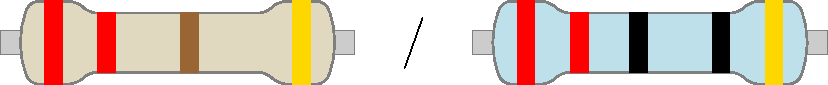
\includegraphics[width=0.5\textwidth]{kuvat/220.pdf}
    \item Koekytkentälevy
    \item Arduino UNO (jännitelähteenä)
    \item LED
    \item Hyppylankoja
\end{itemize}
\end{tcolorbox}
\end{minipage}
\begin{minipage}{0.5\textwidth}
\begin{tcolorbox}[colback=blue!10,title=Piirin toiminta,colbacktitle=purple!90]
LEDin harjoituskytkentä. LED palaa, kun piiri on kytketty jännitelähteeseen.
\tcblower
\begin{center}
\begin{tikzpicture}
\ctikzset{american}
\draw (0,0) to[R,l=$220\Omega$] (0,-2) to [led] (0,-4);
\draw (-2,0) to[V,l=$5V$] (-2,-4); 
\draw (-2,0) to[short] (0,0);
\draw (-2,-4) to[short] (0,-4);
\end{tikzpicture}
\end{center}
\end{tcolorbox}
\end{minipage}

\begin{tcolorbox}[colback=red!10,colbacktitle=red,title=HUOM!]
Aina kun rakennat tai muutat piiriä, pidä Arduino irrotettuna tietokoneesta! 
\tcblower
LEDin kanssa kytketään aina sarjaan vastus (nyt $220\Omega$), kun kytket LEDin $5V$- jännitteeseen.
\end{tcolorbox}

\begin{tcolorbox}[title=Vastuksen arvo]
Jos sinulla ei ole käytössä yleismittaria oikean vastuksen arvon mittaamiseen, tai haluat harjoitella vastusten värikoodien lukemista, vastusten värikoodit löydät sivulta \pageref{varikoodit}.

Nyt tarvitaan $220\Omega$ vastus eli jompikumpi alla olevista vaihtoehdoista:

\begin{center}
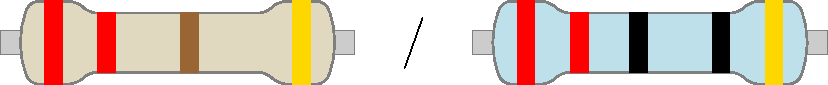
\includegraphics[width=0.5\textwidth]{kuvat/220.pdf}
\end{center}
\end{tcolorbox}

\begin{tcolorbox}[title=LEDin kytkeminen,colback=blue!10,colbacktitle=purple!90]\label{box:led}
Huomaa, että on merkitystä kummin päin LED kytketään koekytkentälevylle! 

LEDissä on kaksi jalkaa, joista toinen on pidempi. LEDin muovi on toiselta puolelta kaareva, ja toiselta siinä on suora leikkaus, lyhyempi jalka on suoran leikkauksen puolella. Lyhyemmän jalan nimi on katodi ja pidemmän jalan anodi.

\begin{minipage}{0.5\textwidth}
Piirrosmerkissä:
\begin{center}
\begin{tikzpicture}
%\node at (-1,0) {anodi};
\draw (0,0) node[left,text width=1.5cm] {anodi\\ pitkä jalka} to[led,o-o] (2,0) node[right,text width=2cm] {katodi\\lyhyt jalka};
\end{tikzpicture}
\end{center}
\end{minipage}
\begin{minipage}{0.5\textwidth}
\begin{tikzpicture}
\node (led) at (0,0) {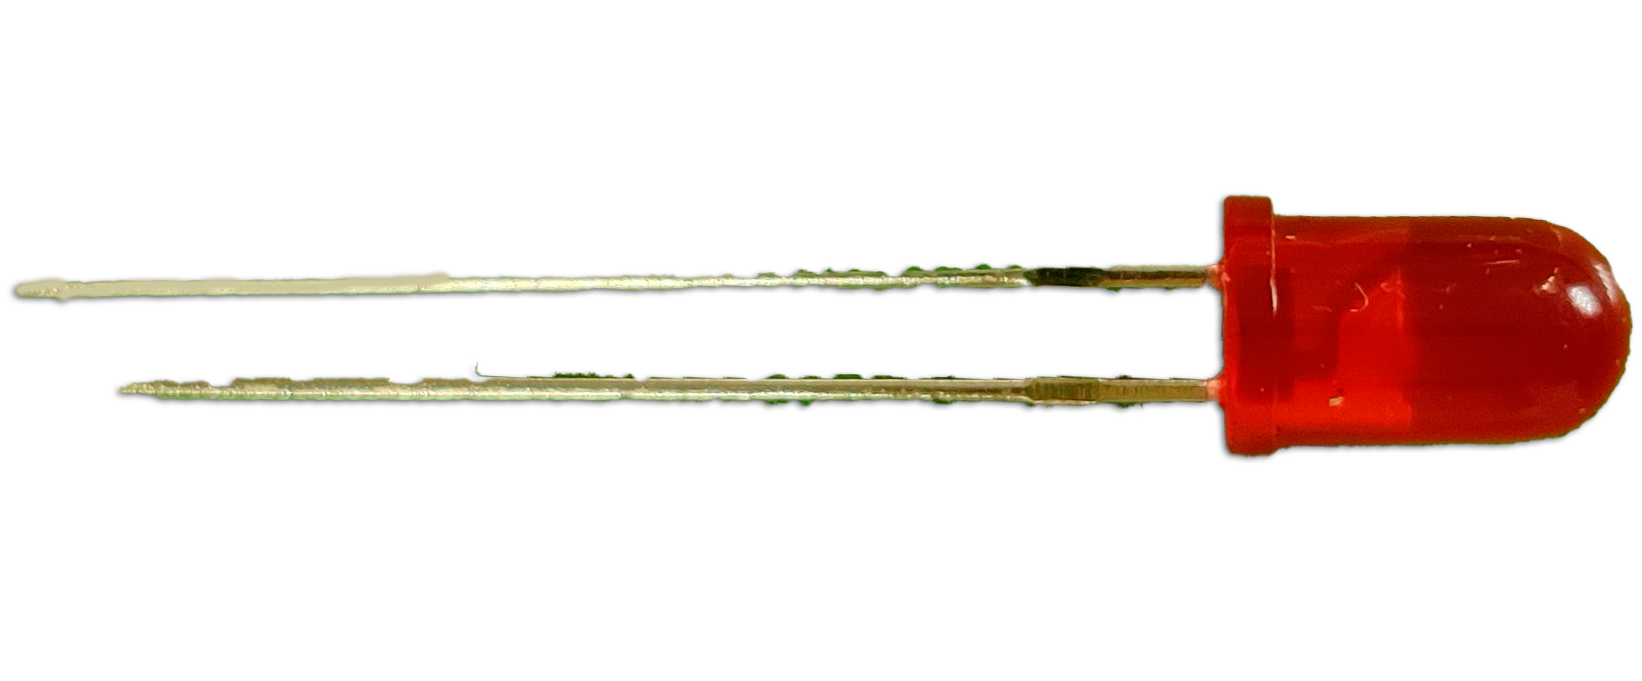
\includegraphics[width=0.95\textwidth]{kuvat/led.png}};
\node[above=0.5] (led) {Anodi (pitkä jalka)};
\node[below=0.5] (led) {Katodi (lyhyt jalka) + tasainen puoli};
\end{tikzpicture}
\end{minipage}

LED, eli valoa säteilevä diodi päästää virtaa läpi vain toiseen suuntaan kuten diodit. Jos anodille kytketään tarpeeksi suuri jännite verrattuna katodiin, virta kulkee ja valo palaa. Jos taas katodilla on suurempi jännite kuin anodilla, virtaa ei kulje ja LED ei pala. Jos anodilla ei ole tarpeeksi suuri jännite verrattuna katodiin, virta ei kulje. Riippuen LEDistä, vaadittu kynnysjännite voi vaihdella ja on tyypillisesti 1,5-4,5 volttia. 
\end{tcolorbox}

\begin{tcolorbox}[title=Jännitelähteen kytkeminen]
Jännitelähde on Arduinossa sisäänrakennettuna. Jotta voimme kytkeä jännitelähteen piiriin, tarvitsemme jännitelähteen molemmat päät: +5V ja maan (GND), kytkemällä vain toinen piiriin emme saa aikaan haluttua vaikutusta.

Arduino levyllä on kolme eri GND-riviä, ja mikä tahansa niistä käy. Kuvassa selvyyden vuoksi ne on numeroitu.

\begin{minipage}{0.3\textwidth}
\begin{tikzpicture}
\ctikzset{american}
\draw (-2,0.5) node[above] {5V} to[short,o-]  (-2,0) to[V,l=$5V$] (-2,-2) to[short,-o] (-2,-2.5) node[below] {GND};
%\node (-2,0.5) {5V};
\end{tikzpicture}
 \end{minipage}
\begin{minipage}{0.7\textwidth}
\begin{tikzpicture}[scale=0.5]
\pic[scale=0.2] at (0,0) {myarduino};
\draw[red,wire] (Ar5V) to[short,*-o] ++(-5,0) node[left,black] {5V};
\draw[black,wire] (ArGND2) to[short,*-o] ++(-5,0) node[left,black] {GND};
\end{tikzpicture}
\end{minipage}
\end{tcolorbox}

%\begin{tcolorbox}[colback=yellow!10, title={Tee kytkentä!},colbacktitle=orange]
Kytketään ensin vastus ja LED kuvan mukaisesti ja lisätään kaksi hyppylankaa.

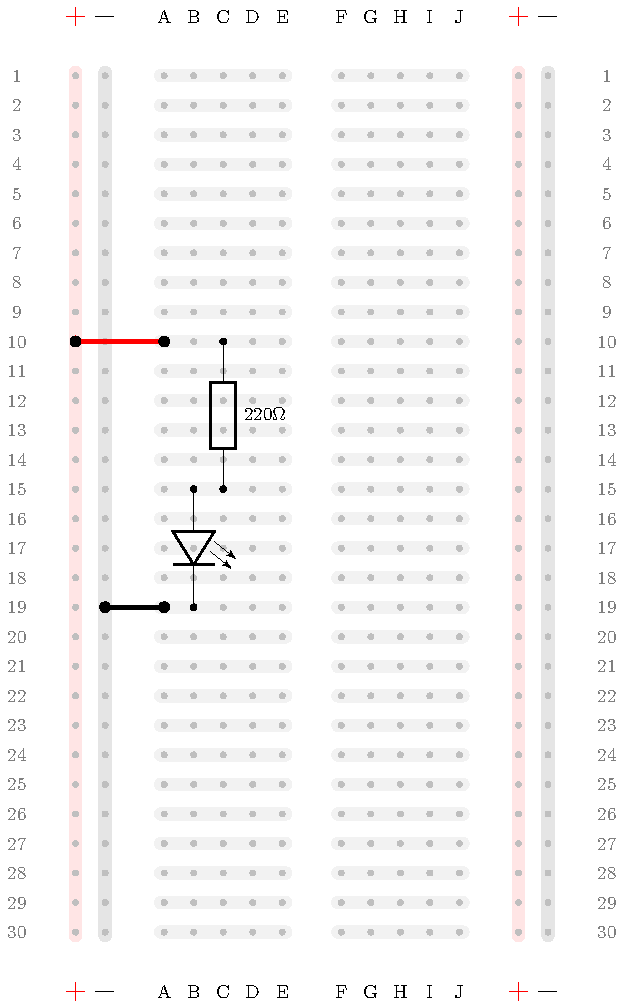
\includegraphics[width=0.8\textwidth]{kuvat/kuva4.pdf}


Nyt on siis tehty muuten kytkennät ja pitää kiinnittää vielä jännitelähde piiriin.
%\end{tcolorbox}

Kytketään nyt käyttöjännite (+5V) vasemmalle $+$ pystyriville ja maa (GND) tämän viereiselle $-$ pystyriville.

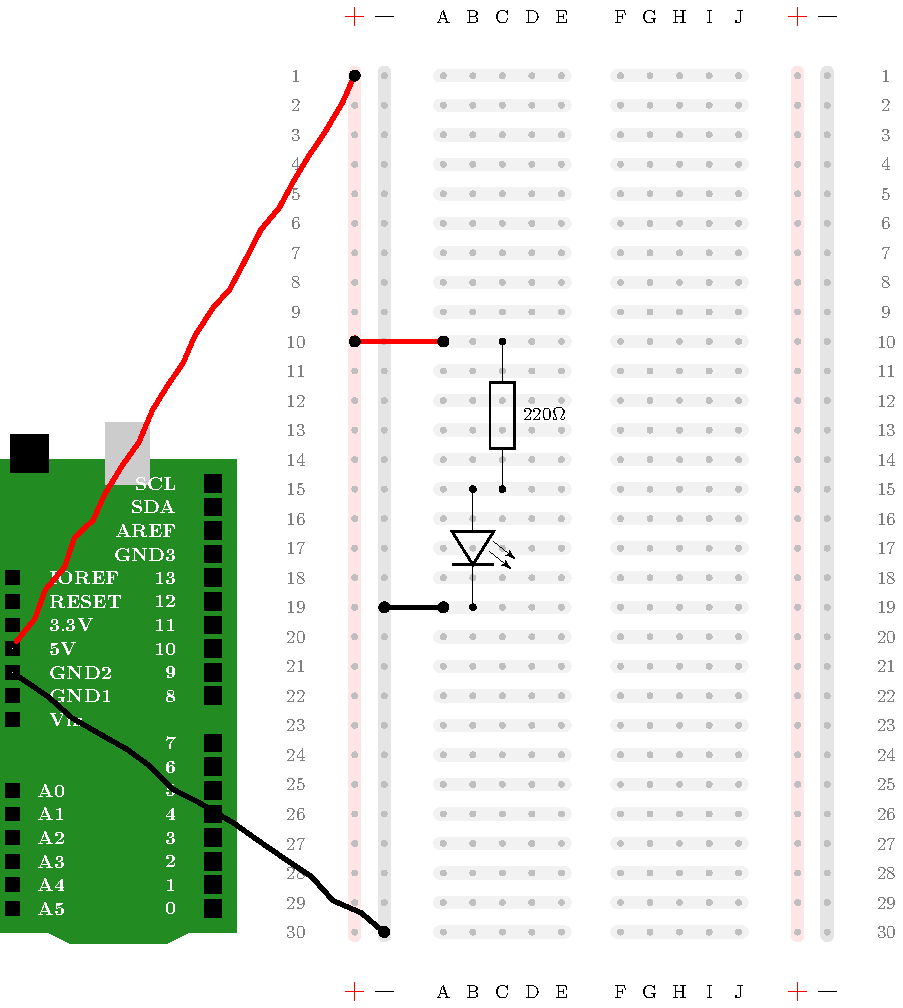
\includegraphics[width=0.95\textwidth]{kuvat/kuva5.pdf}

Nyt kun yhdistetään Arduino johdolla tietokoneeseen, LED syttyy!

\section{Lisätään kytkentään painonappi}

\begin{minipage}{0.5\textwidth}
\begin{tcolorbox}[colback=lime!10,title=Tarvikkeet, colbacktitle=green!10,coltitle=black]
\begin{itemize}
    \item Edellisen työn koottu piiri
    \item Painonappi
\end{itemize}
\end{tcolorbox}
\end{minipage}
\begin{minipage}{0.5\textwidth}
\begin{tcolorbox}[colback=blue!10,title=Piirin toiminta,colbacktitle=purple!90]
Painonapin koekytkentä. Nappia painamalla LED syttyy.
\tcblower
\begin{center}
\begin{tikzpicture}
\ctikzset{american}
\draw (0,0) to[R,l=$220\Omega$] (0,-2) to [led] (0,-4);
\draw (-2,0) to[V,l=$5V$] (-2,-4); 
\draw (-2,0) to[nopb] (0,0);
\draw (-2,-4) to[short] (0,-4);
%\draw (-2,0) to[nopb] (-2,3);
\end{tikzpicture}
\end{center}
\end{tcolorbox}
\end{minipage}

\begin{tcolorbox}[colback=red!10,colbacktitle=red,title=HUOM!]
Aina kun rakennat tai muutat piiriä, pidä Arduino irrotettuna tietokoneesta! 
\end{tcolorbox}

Nyt lisätään piiriin painonappi. 

\begin{tcolorbox}[title=Painonapin kytkeminen,colback=blue!10,colbacktitle=purple!90]
Arduinon mukana tulevassa painonapissa on neljä pinniä, ja asetetaan keskellä olevan uran ylitse. Jos nappia ei paineta, niin A-E ja F-J rivillä 2 ovat samaa pistettä, mutta eri pistettä kuin rivin 4 (A-E) ja (F-J). Jos nappia painetaan, niin molempien rivien (2 ja 4) kaikki pisteet ovat kiinni toisissaan.


\begin{tikzpicture}[scale=0.5]
\BREADBOARD (0,0) {5};
\draw[thick,fill=hopea] (E2.east) rectangle (F4.west) coordinate[pos=0.5] (Y);
\draw[fill=black] (Y) circle (0.5);
\draw (E2.east) to[short,*-*] (E2);
\draw (E4.east) to[short,*-*] (E4);
\draw (F4.west) to[short,*-*] (F4);
\draw (F2.west) to[short,*-*] (F2);
\end{tikzpicture}
\end{tcolorbox}

Siirretään lyhyempää punaista johtoa kohdasta A10 kohtaan A8. Lisätään painonappi pisteisiin E8, E10, F8 ja F10.

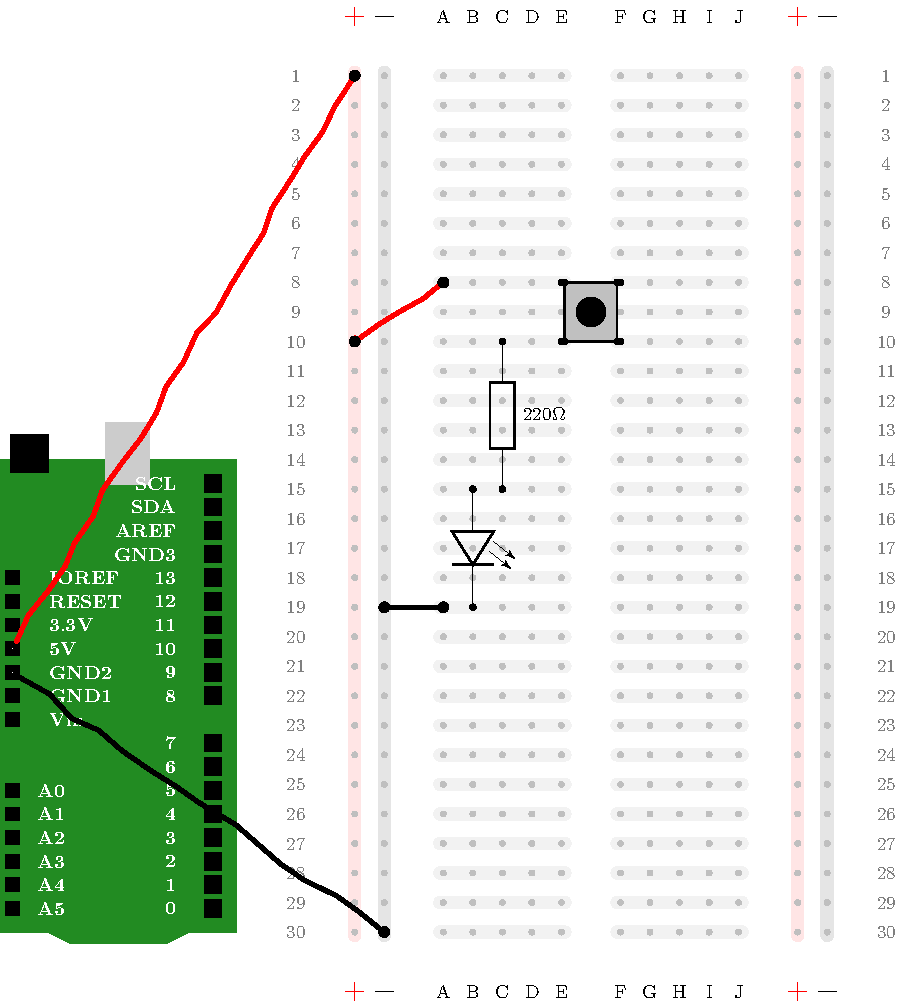
\includegraphics[width=0.95\textwidth]{kuvat/kuva6.pdf}

Nyt kytke Arduino takaisin kiinni koneeseen, ja saat LEDin syttymään painamalla nappulaa. 

